% Vorlage für eine Bachelor- oder Masterthesis
%% Dipl.-Ing. Stefan Averkamp
%% Version 2.5
%% 18.03.2021
%% ----------------------------------------------------------------------------

\documentclass[
cmyk,
pdftex,
a4paper,           % DinA4 Papier
%12pt,             % Schriftgröße
oneside,           % oneside, twoside
openright,         % openleft, openright, openany
numbers=noenddot,  % keinen Punkt hnter Kapitel- oder Sectionnummern
chapterprefix=off, % Kapitel wird vor die Kapitelnummer geschrieben
]{scrbook}
\sloppy
%% Preambel einbinden -----------------------------------------------------------------------------
\UseRawInputEncoding
\setcounter{secnumdepth}{3}         % 3 levels in section numbering

%% Useful packages -------------------------------------------------------------------------------
\usepackage[english]{babel}         % English language
\usepackage{scrhack}
\usepackage{placeins}
\usepackage{subcaption}
\usepackage{lmodern}
\usepackage{cmbright}
\usepackage{enumitem}               % Package for customized lists
\usepackage[OT1]{fontenc}
\usepackage{blindtext}              % Use \blindtext to insert dummy text
\usepackage{mdwlist}                % More compact lists with itemize and co
\usepackage{graphicx}               % Graphics
\usepackage{epstopdf}               % Automatically convert eps images to pdf
\usepackage{ltxtable}               % Combines longtable and tabularx
\usepackage{multirow}               % Multi-row cells in tables
\usepackage[dvipsnames,table,xcdraw]{xcolor}  % Alternating colors in tables
\usepackage{rotating}               % Rotate text and other elements
\usepackage{multicol}               % Multicolumn formatting
\usepackage{amsmath}                % Mathematical formulas
\usepackage{amsthm}                 % Theorem style
\usepackage{mathtools}
\usepackage{amssymb}                % Mathematical symbols
\usepackage{wrapfig}                % Wrapping figures
\usepackage{float}                  % For [h!] or [H] positioning
\usepackage{booktabs}               % For tables from Excel to LaTeX
\usepackage{eurosym}                % Use Euro symbol
\usepackage{url}                    % URLs
\usepackage{etoolbox}
\appto\UrlBreaks{\do\a\do\b\do\c\do\d\do\e\do\f\do\g\do\h\do\i\do\j
    \do\k\do\l\do\m\do\n\do\o\do\p\do\q\do\r\do\s\do\t\do\u\do\v\do\w
    \do\x\do\y\do\z}
\usepackage{adjustbox}
\usepackage{fancybox}               % Boxes and frames
\usepackage{caption}                % Extended settings for captions
\usepackage{array}                  % Extended options for arrays and tables
\usepackage{icomma}                 % Reduces space after comma in decimal numbers
\usepackage{setspace}               % Define line spacing

%% PDF options (links and more) -----------------------------------------------------------------
\usepackage{pdfpages}
\usepackage[utf8]{inputenc}         % UTF-8 encoding
\usepackage[english=british]{csquotes}
\usepackage[pdftex, raiselinks, pdfpagelabels, hypertexnames=false, pdfstartview={Fit}]{hyperref}
\definecolor{lightblue}{rgb}{0.9,0.9,1}

%% PDF metadata
\hypersetup{
    pdfauthor = {Nico Bierbaum},
    pdftitle =  {Scientific Work},
    pdfsubject = {Density and Shrinkage Evaluation of 316L Printed Parts in the FDM Process},
    pdfkeywords = {3D printing, filament, metal, density, tensile test, shrinkage},
    pdfcreator = {LaTeX with hyperref package}
}

%% Header and footer -----------------------------------------------------------------------------
\usepackage[headsepline]{scrlayer-scrpage}
\pagestyle{scrheadings}
\clearpairofpagestyles
\ihead{\headmark} % Redefine
\ohead{\pagemark}

%% Page margins -----------------------------------------------------------------------------------
\usepackage[a4paper,inner=4cm,outer=2.5cm,top=2cm,bottom=2cm,includeheadfoot]{geometry}

%% Bibliography -----------------------------------------------------------------------------------
\usepackage[style=numeric-comp,sorting=none,backend=biber]{biblatex}

\DeclareFieldFormat{labelalpha}{\textsc{#1}}    % Sets the author in small caps 
\renewcommand*{\mkbibnamefamily}[1]{\textsc{#1}}  % Sets the last name in small caps 
\renewcommand*{\mkbibnamegiven}[1]{\textsc{#1}}  % Sets the first name in small caps 
\renewcommand*{\mkbibnameprefix}[1]{\textsc{#1}}  % Sets the prefix in small caps 
\DeclareFieldFormat{title}{``#1''}      % Sets the title in quotation marks
\DeclareFieldFormat{date}{({#1})}               % Sets the date in parentheses
\makeatletter
\def\blx@maxline{77}
\makeatother
\addbibresource{LiteratureDB.bib} % Load bibliography

%% Glossary and abbreviations ---------------------------------------------------------------------
\usepackage{nomencl}
% English title
\renewcommand{\nomname}{Glossary and List of Abbreviations}
% Dots between abbreviation and explanation
\setlength{\nomlabelwidth}{.20\hsize}
\renewcommand{\nomlabel}[1]{#1 \dotfill}
% Reduce line spacing
%\setlength{\nomitemsep}{-\parsep}
\makenomenclature
\setlength{\headsep}{1.5\baselineskip}

%% ---------------------------------------------------------------------------------------------------
%% Create glossary and abbreviations: ------------------------------------------------------------------
%% 1. Run LATEX
%% 2. Open a command prompt and navigate to the folder with the "thesis.tex" file.
%% 3. Run the command   makeindex thesis.nlo -s nomencl.ist -o thesis.nls
%% 4. Run LATEX again. The glossary and abbreviations should now be present.

%% Source code -------------------------------------------------------------------------------------
\usepackage{listings}
\lstset{ %
    basicstyle=\scriptsize,         % the size of the fonts that are used for the code
    numbers=left,                   % where to put the line-numbers
    numberstyle=\footnotesize,      % the size of the fonts that are used for the line-numbers
    backgroundcolor=\color{white},  % choose the background color. You must add \usepackage{color}
    commentstyle=\color{green},
    stringstyle =\color{orange},
    xleftmargin=1.5em,
    xrightmargin=1em,
    frame=tb,                       % adds a frame around the code
    tabsize=2,                      % sets default tabsize to 2 spaces
    captionpos=b,                   % sets the caption-position to top or bottom
    breaklines=true,                % sets automatic line breaking
    breakatwhitespace=false         % sets if automatic breaks should only happen at whitespace
    literate =%
     {#}{\#}1
}
\renewcommand*{\lstlistingname}{Source Code}
\renewcommand*{\lstlistlistingname}{List of Source Codes}

%% Tikz for (complex) colorful drawings ---------------------------------------------------------
\usepackage{tikz}
\usetikzlibrary{positioning,mindmap,shapes,shapes.multipart,shadows,arrows,patterns,topaths}
\usepackage{pgfplots}
\pgfplotsset{width=7cm,compat=newest}

\definecolor{yellow}{HTML}{FFFCCC}
\definecolor{green}{HTML}{CFFFCC}
\definecolor{blue}{HTML}{CCE9FF}
\definecolor{darkblue}{HTML}{99b7EE}
\definecolor{red}{HTML}{FFA8A8}
\definecolor{orange}{HTML}{FFD28F}

\lstset
{
    breaklines=true,
    tabsize=3,
    showstringspaces=false
}

\lstdefinestyle{Common}
{
    extendedchars=true,
    language={[Visual]Basic},
    frame=single,
    %===========================================================
    framesep=3pt,%expand outward.
    framerule=0.4pt,%expand outward.
    xleftmargin=3.4pt,%make the frame fits in the text area. 
    xrightmargin=3.4pt,%make the frame fits in the text area.
    %=========================================================== 
    rulecolor=\color{Red}
}

\lstdefinestyle{A}
{
    style=Common,
    backgroundcolor=\color{Yellow!10},
    basicstyle=\scriptsize\color{Black}\ttfamily,
    keywordstyle=\color{Orange},
    identifierstyle=\color{Cyan},
    stringstyle=\color{Red},
    commentstyle=\color{Green}
}

\lstdefinestyle{B}
{
    style=Common,
    backgroundcolor=\color{Black},
    basicstyle=\scriptsize\color{White}\ttfamily,
    keywordstyle=\color{Orange},
    identifierstyle=\color{Cyan},
    stringstyle=\color{Red},
    commentstyle=\color{Green}
}

\begin{document}

%% Titelseite einbinden ---------------------------------------------------------------------------
\thispagestyle{empty}
\newgeometry{
	top=25mm, 
	bottom=7mm,
	left=46mm,
	right=36mm
}
%Logos------------------------------------------------------------------------------
%Logos bekommen eine definierte Breite von 6cm, die Box in der das Logo ist, ist 7cm
\vspace*{-2cm} %evtl nützlich um logos weiter oben zu platzieren
\setlength{\unitlength}{1cm}
\hfill
%% Firmenlogo ----------------------------------------------------------------------
\begin{minipage}[t]{14cm}
\begin{minipage}[t]{7cm}

\end{minipage}
%% FH-Logo ----------------------------------------------------------------------
\begin{minipage}[t]{7cm}
   \begin{flushright}
    
\includegraphics[width=66mm]{bilder/fhm_Logo_CMYK_30mm.pdf}
   \end{flushright}
\end{minipage}\\
\end{minipage}
%-----------------------------------------------------------------------------------

\begin{minipage}[t]{11cm}
\vspace{2cm}					
\begin{Huge}
\begin{center}\textsf{\textbf{Wissenschaftliche Arbeit}}\end{center}
\end{Huge}


\vspace{2cm} 								
\begin{Large}
\hfill 
\begin{center}

\begin{large}
	Nico Bierbaum
\end{large}

\vspace{2cm} %3cm
%\begin{minipage}[t][2.5cm]{14cm}
\begin{flushright}
	\hfill{Analyse der Dichte und Schwindung sowie Ermittlung mechanischer Kennwerte von Edelstahlkomponenten, hergestellt mittels 3D-Druck im FDM-Verfahren}\\
\end{flushright}			
%\end{minipage}
\end{center}	
\end{Large}

\begin{large}
\vspace{30mm}  %3cm
%\begin{minipage}[t][1.5cm]{14cm}
\hfill Betreuer der Arbeit: Prof. Dr.-Ing. Hilmar Apmann

\hfill Steffen Florian M.Sc.\\
%\end{minipage}
\end{large}

\vspace{35mm}
\hfill Steinfurt, den \today
\end{minipage}
\vspace{20mm}

\begin{minipage}[t]{136.5mm}
\begin{flushright}

\includegraphics[width=82mm]{bilder/MB_CMYK.pdf}
\end{flushright}
\end{minipage}
\restoregeometry
%--------------------------------------------------------------------------------------------------------

%% Sperrvermerk, Eidesstattliche Erklärung, Vorwort -----------------------------------------------
\frontmatter

\pagestyle{scrheadings}
\pagenumbering{Roman}


\input{inhalt/Sperrvermerk.tex}
%Eidesstattliche Erklärung-------------------------------------------------------------------------------
\chapter*{Eidesstattliche Erklärung}
\addcontentsline{toc}{chapter}{Eidesstattliche Erklärung}

Ich erkläre hiermit an Eides statt, dass ich die vorliegende Hausarbeit selbstständig und ohne unzulässige fremde Hilfe angefertigt habe. Die verwendeten Literaturquellen sind im Literaturverzeichnis vollständig zitiert.





\vspace{6cm}
Steinfurt, \today

% Vorwort -----------------------------------------------------------------------------------------
\chapter*{Vorwort}

Schreiben wir den Bums hier ein bisschen wie Werbung oder soll das komplett sachlich und nüchtern passieren?

\addcontentsline{toc}{chapter}{Vorwort}



%% Inhaltsverzeichnis einbinden -------------------------------------------------------------------
\pdfbookmark[0]{Inhaltsverzeichnis}{tableofcontents}
\tableofcontents

%% Verzeichnisse einbinden  -----------------------------------------------------------------------
\listoffigures              %% Abbildungsverzeichnis
\listoftables               %% Tabellenverzeichnis
\lstlistoflistings          %% Quelltextverzeichnis
\nomenclature{AM}{Additive Fertigung \textit{engl. Additive Manufacturing}}
\nomenclature{CAD}{rechnerunterstütztes Konstruieren \textit{engl. Computer Aided Design}}
\nomenclature{FDM}{Schmelzschichten \textit{engl. Fused Deposit Modeling}}
\nomenclature{CNC}{rechnergestützte numerische Steuerung \textit{engl. Computer Numerical Control}}
\nomenclature{SLM}{selektives Laserschmelzen \textit{engl. Selective Laser Melting}}
\nomenclature{PTFE}{Polytetrafluorethylen}
\nomenclature{Heizblock}{Baugruppe aus Heizelement und Druckdüse}
\nomenclature{PLA}{Polylactide}
\nomenclature{PETG}{Polyethylenterephthalat}
\nomenclature{ABS}{Acrylnitril-Butadien-Styrol-Copolymer - Thermoplast}
\nomenclature{Firmware}{Software, die in elektronische Geräte fest implementiert ist}
\nomenclature{Open-Source}{Software, deren Quellcode frei verfügbar ist und von unabhängigen Dritten eingesehen und editiert werden kann}
\nomenclature{Software}{Begriff für Programme auf technischen Geräten}




\cleardoublepage% or \clearpage
\markboth{\nomname}{\nomname}

\printnomenclature
% \addcontentsline{toc}{chapter}{Glossar und Abkürzungsverzeichnis}
  %% Abkuerzungsverzeichnis
%% Eigentlicher Inhalt der Arbeit -----------------------------------------------------------------
%% Einbinden der einzelnen Kapitel. Jedes Kapitel in eine seperate Datei speichern. ---------------
\mainmatter
\chapter{Einleitung}
\label{einleitung}

\subsection*{Disclaimer zur Verwendung des generischen Maskulinums}
Für die Lesbarkeit und bessere Verständlichkeit dieses Businessplans haben wir uns dazu entschieden, das generische Maskulinum zu verwenden. Wir möchten darauf hinweisen, dass wir damit keinesfalls eine Diskriminierung oder Geringschätzung von Personen anderer Geschlechter beabsichtigen. Selbstverständlich sind alle im Text verwendeten Bezeichnungen geschlechtsneutral zu verstehen und gelten gleichermaßen für Frauen und Männer.

\pagebreak

\section{Hintergrund und Motivation}
Additive Fertigung \textit{engl. Additive Manufacturing (AM)} wurde in den 1990ern eingeführt und beschreibt eine bis dahin neuartige Technologie 3D-Objekte in einem Schicht-für-Schicht Verfahren zu fertigen. Im Gegensatz zur additiven Fertigung [AM] steht die subtraktive Fertigung, auch als konventionelle Fertigung bezeichnet. Bei der die gewünschten Bauteile durch Abtrag von Material (z.B. beim Fräsen oder Drehen) hergestellt werden. Durch die additive Fertigung ergibt sich eine hohe Flexibilität und Designfreiheit, dies ist insbesondere für Prototypenherstellung, als auch immer mehr in der Serienproduktion von Bedeutung \autocite{Prof.Dr.Ing.ChristianSeidel.2023}.
Zu Beginn ist diese Technologie hauptsächlich in der Prototypenphase eingesetzt, da sich die Materialienauswahl auf Polymere beschränkt. So gab es vor allem viele Kunststoffe zur Auswahl, aber keine Materialien, die einem Stahl gleichkommen.
Heute ist AM im weiteren Sinne auch für die Herstellung von funktionellen Teilen eingesetzt.  Firmen aus den Bereichen Luft- und Raumfahrt, Automobilherstellung, Energie und Medizin sind interessiert an dem Einsatz der AM zur Herstellung verschiedener Bauteile.
AM bringt folgende Vorteile mit sich:
\begin{itemize}
    \item Große Freiheit im Design der Bauteile, was eine individuelle Anpassung an die Produktion ermöglicht. Zudem ist die Erstellung komplexer Bauteile deutlich einfacher als mit konventionellen Methoden.
    \item Der Konstruktionsprozess und die Prototypenphase sind deutlich schneller. Einzelne Prozessschritte sind schneller.
\end{itemize}

1.1 Hintergrund und Motivation\\
1.2 Zielsetzung der Arbeit\\
1.3 Aufbau der Arbeit
\chapter{Stand der technik}
\section{Methoden zur Charakterisierung von (Bag-)Mischsysteme}
\subsection{Charakterisierungsaspekte - Leistungseintrag, Suspension, Mischzeit, Scherstress, …}
\subsection{Auswertemethoden - u.a. bildbasierte Auswertemethoden}
\section{Roboterbasierte (Bag-)Mischsystemen}
\chapter{Anforderungsanalyse}
\chapter{Systementwurf}

\section{Symbolverzeichnis}


\begin{table}[htbp]
    \centering
    \begin{tabular}{l l}
        \hline
        \textbf{Symbol/Formelzeichen} & \textbf{Beschreibung} \\
        \hline
        \((KS)_E\) & Ursprung des Koordinatensystems auf der schiefen Ebene \\
        \( _{(E)}\vec{p}(t) \) & 3D-Vektor der Gesamtbewegung in Ebene \((KS)_E\)\\
        \(_{(E)}\vec{p_B} (t) \) & 3D-Vektor der reinen Bewegung in Ebene \((KS)_E\) \\
        \(_{(E)}\vec{p_0}\) & 3D-Startvektor. Durch Eingabe des Nutzers (Spaltbreite)\\
        \(z(t)\) & Bewegungsgleichung der Robotertrajektorie \\
        \(\hat{z}\) & Eingabe des Benutzers für die Hubhöhe\\
        \(\omega\) & Kreisfrequenz \\
        \(f\) & Eingabe des Nutzers für die Frequenz \\
        \(W\) & Physikalische Arbeit \\
        \(F\) & Physikalische Kraft \\
        \(P\) & Physikalische Leistung \\
        

        \hline
    \end{tabular}
    \caption{Symbol- und Formelzeichenverzeichnis}
\end{table}

\section{Bewegungsprofil des Paddel-Mischers}

\begin{figure}[h]
    \centering
    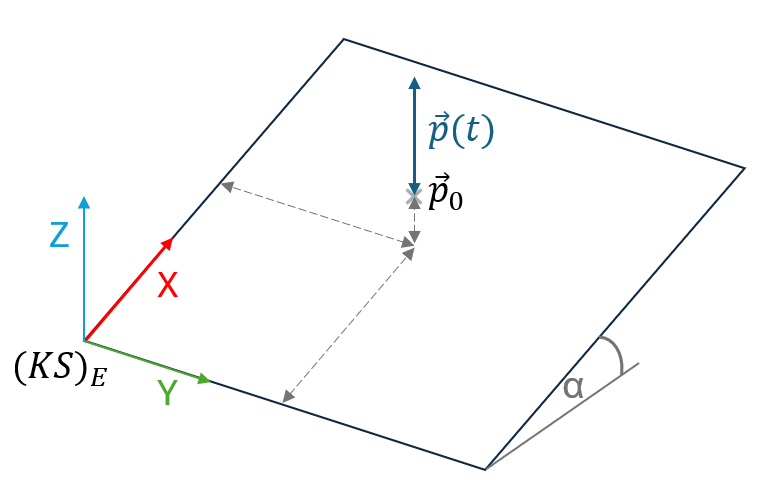
\includegraphics[width=0.8\textwidth]{bilder/KS_E-Koordinatensystem_Ebene.png}
    \caption[Visualisierung des Koordinatensystems auf der schiefen Ebene]{Visualisierung des Koordinatensystems auf der schiefen Ebene (eigene Darstellung)}\label{fig:VisualisierungKoordinatensystemSchiefe}
\end{figure}

\noindent Im Folgenden werden die drei Parameter zur reproduzierbaren Beschreibung der Paddel Bewegung in allen drei Bewegungsrichtungen beschrieben. Hierbei ist \( _{(E)}\vec{p}(t) \) stellvertretend für die Gesamtbewegung in Koordinatensystem \((KS)_E\). \(_{(E)}\vec{p_B} (t) \) beschreibt die veränderliche Position ausgehend von \(_{(E)}\vec{p_0}\).\\

\textbf{Allgemein:}


\begin{equation}
    \begin{aligned}
        _{(E)}\vec{p}(t) &= _{(E)}\vec{p_B}(t) + _{(E)}\vec{p_0}\\
        \text{mit}\\
        _{(E)}\vec{p}_B(t) &= _{(E)}\left(x_B(t), y_B(t), z_B(t)\right)\\
        _{(E)}\vec{p_0} &= _{(E)}\left(x_0, y_0, z_0\right)
    \end{aligned}
    \label{eq:generelleBewegung}
\end{equation}

\autoref{eq:generelleBewegung} ist unabhängig von der eingeleiteten Bewegungsform und Richtung. Es können in \(\vec{p}_B(t)\) alle möglichen Bewegungsformen dargestellt werden.\\

Hier folgt nun die Errechnung anhand einer sinus-förmigen Bewegung entlang der Z-Achse:

\begin{equation}
    \begin{aligned}
        _{(E)}\vec{p}_{0} &= (x_{0}, y_{0}, z_{0})\\
        _{(E)}\vec{p}(t) &= (x, y, z(t)) + \vec{p}_{0}  
    \end{aligned} 
\end{equation}

\( z(t) \) ist definiert durch:

\begin{equation}
    z(t) = -\hat{z}(\cos(\omega t)-1)  \quad \text{mit} \quad \hat{z} = \frac{h}{2}
\end{equation}

und \( \omega = 2 \pi f = \frac{2 \pi}{T} \).

Zum Beispiel, bei \( t = 0 \):

\begin{equation}
    z(0) = -\hat{z}(1-1) = 0
\end{equation}

Beispiel bei \( t = \frac{1}{4}T \):

\begin{equation}
    \begin{aligned}
        z\left(\frac{1}{4}T\right) &= -\hat{z}\left(\cos\left(\frac{2\pi T}{T \cdot 4}\right) - 1\right) \\
        &= -\hat{z}\left(\cos\left(\frac{\pi}{2}\right) - 1\right) \\
        &= -\hat{z}(0 - 1) = \hat{z} = \frac{1}{2} h
    \end{aligned}
\end{equation}

Und bei \( t = \frac{1}{2}T \):

\begin{equation}
    \begin{aligned}
        z\left(\frac{1}{2}T\right) &= -\hat{z}\left(\cos\left(\frac{2\pi T}{T \cdot 2}\right) - 1\right) \\
        &= -\hat{z}\left(\cos(\pi) - 1\right) \\
        &= -\hat{z}(-1 - 1) = 2\hat{z} = h
    \end{aligned}
\end{equation}


wobei \( _{(E)}\vec{p(t)} \) die Bewegung des Paddel-Mittelpunkts und \( _{(E)}\vec{p}_{0} \) den Mittelpunkt auf dem Einwegbeutel repräsentiert.

\begin{figure}[h]
    \centering
    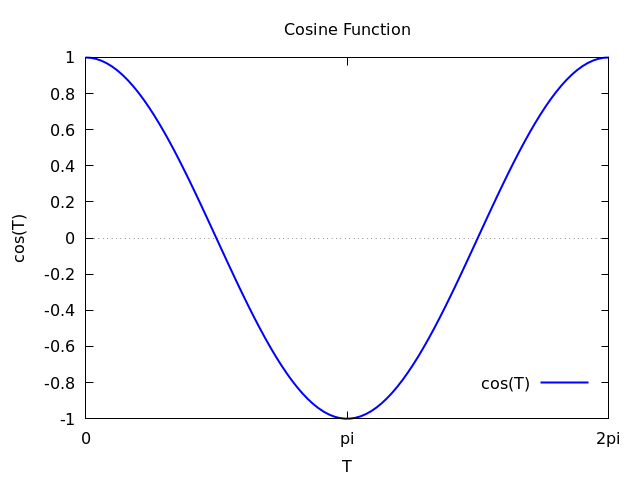
\includegraphics[width=0.8\textwidth]{bilder/cosine-plot.png}
    \caption[Kosinusfunktion]{Klassische Kosinusfunktion (\( cos(t) \)) (eigene Darstellung)}\label{fig:Kosinusfunktion}
\end{figure}
\FloatBarrier

\begin{figure}[h]
    \centering
    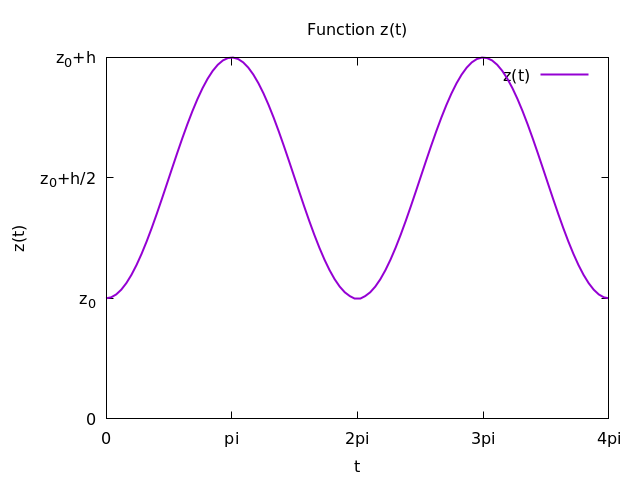
\includegraphics[width=0.8\textwidth]{bilder/cosine-plot_real.png}
    \caption[Darstellung der Paddelbewegung anhand der Cosinusfunktion]{Darstellung der Paddelbewegung in Z-Richtung anhand der Cosinusfunktion \( z(t) = -\hat{z}(\cos(\omega t)-1) \) (eigene Darstellung)}\label{fig:PaddelbewegungCos}
\end{figure}
\FloatBarrier



Beispiel Sinus-Bewegung in \( _{(E)}\) Z-Richtung:
\begin{equation}
    \begin{aligned}
        x &= x_B + x_0\\
        y &= y_B + y_0\\
        z(t) &= \hat{z}\left( 1 - \cos(\omega t) \right) +z_0\\
        \text{mit}\\
        &\hat{z} = 2h\\
        &\omega = 2\pi f
    \end{aligned}
\end{equation}

\section{Definition der Leistungseinbringung für den Mischprozess}

Allgemein gilt:

\begin{equation}
    W = \int_{t_1}^{t_2} \vec{F}(\vec{s(t)})\cdot d \vec{s}
\end{equation}

\noindent Wenn die Kraftrichtung der Bewegungsrichtung gleicht und beide Vektoren in dieselbe Richtung zeigen gilt:

\begin{equation}
    W = F \cdot s \text{   und   } P = \frac{W}{dt}
\end{equation}

\noindent In unserem Fall zeigt die Kraft \(F_z\) in die Bewegungsrichtung \(z\), aber sie ist nicht konstant. Daher gilt:

\begin{equation}
    \begin{aligned}
        W = \int_{t_1}^{t_2} F_z (z(t))\cdot dz\\
        W = \int_{t_1}^{t_2} F_z (t)\cdot dz
    \end{aligned}
\end{equation}

Der Zusammenhang von Kraft und Weg ist in \autoref{fig:EingebrachteLeistungWegZeit} dargestellt. Bei \(z_0\) liegt die maximale Kraft an, da der Abstand zum Einwegbeutel am geringsten ist.

\begin{figure}[h]
    \centering
    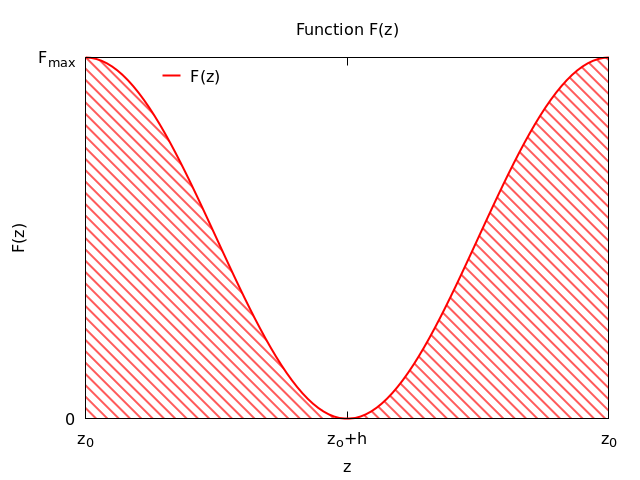
\includegraphics[width=0.8\textwidth]{bilder/force-over-distance.png}
    \caption[Eingebrachte Leistung Weg-über-Zeit-Diagramm]{Eingebrachte Leistung Weg-über-Zeit-Diagramm (eigene Darstellung)}\label{fig:EingebrachteLeistungWegZeit}
\end{figure}
\FloatBarrier

\textbf{Diskrete Messpunkte:}
\begin{equation}
    W = \sum_{t \in \{t_0; t_0 + T; T_0 + 2T; \dots; t_n\}}^{} F_z(t) \cdot \Delta z(t) = \sum_{t \in \{t_0; t_1; \dots; t_n\}}^{} F_z (t) \cdot (z(t+1)-z(t))
\end{equation}
\chapter{Komponentenentwurf}
\section{Software}
\subsection{Parametrisierbares Roboterprogramm zur Ausführung der Bewegung}
\subsection{Entwicklung einer automatisierten Auswerteskriptes}
\subsubsection{zur Auswertung des Leistungseintrages}
\subsubsection{zur Auswertung der Mischzeit bzw. Suspension (z.B. bildbasiert)}
\subsubsection{mit einfacher Bedienbarkeit (für Laboranwender) z.B. mit GUI/Tkinter}
\subsubsection{Generierung von CSV-Daten und Reports}
\section{Hardware}
\subsection{Aufbau einer schrägen im Winkel verstellbar Auflagefläche für den Bag}
\subsection{Aufbau von Sensorik zur Bestimmung der Mischzeit bzw. Suspension (z.B. Kamera + Belichtung unter Bag)}
\chapter{Implementierung (Optional)}
\section{Aufbau und Integration des Gesamtsystems}
\chapter{Validierung/Auswertung}
\section{Durchführung und Dokumentation von Tests zur Validierung der Systemfunktionen gemäß der Anforderungen aus 3.}
\section{Validierung der Systemfunktionen}
\chapter{Auswertemethoden}

%% ...
%%\chapter{Diskursiver Teil}
\label{Zusammenfassung}



%% Beginn vom Anhang ------------------------------------------------------------------------------
\appendix

%% Literaturverzeichnis einbinden. Die Quellen sind in der Datei "LiteraturDB.bib" gespeichert. ---
%% Das Literaturverzeichnis muss vorab über über Tools-->Befehle-->Biber erzeugt werden.--
\begin{flushleft}  % Schaltet den Blocksatz für das Literaturverzeichnis ab.
     \printbibliography
\end{flushleft}
%% Anhang einbinden -------------------------------------------------------------------------------
\chapter{Anhang}
\label{Anhang}

\section{Druckparameter}

\begin{table}[htbp]
    \centering
    \caption{Parametertabelle Prusa MK3S+\newline verwendet für Druck der Würfel und liegenden Zugproben}
      \begin{tabular}{llr}
      \toprule
      \textbf{Parameter} & \textbf{Wert} & \multicolumn{1}{l}{\textbf{Beschreibung}} \\
      \midrule
      Schichthöhe [mm] & \multicolumn{1}{r}{0,1} &  \\
      Drucktemperatur [°C] & \multicolumn{1}{r}{130} &  \\
      Druckgeschwindigkeit [mm/s] & \multicolumn{1}{r}{50} & \multicolumn{1}{p{12.555em}}{Liefert optisch gute Ergebnisse} \\
      Heizbetttemperatur [°C] & \multicolumn{1}{r}{40} &  \\
      Rückzugslänge [mm] & \multicolumn{1}{r}{0,6} & \multicolumn{1}{p{12.555em}}{Standardwert Cura} \\
      Materialflussrate [\%] & \multicolumn{1}{r}{100} &  \\
      Druckoberfläche & Flachkreppband & \multicolumn{1}{p{12.555em}}{Gute Ablöseeigenschaften mit Spachtel} \\
      Prozentsatz Aussenhaut überlappen [\%/mm] & 10/0,04 &  \\
      \bottomrule
      \end{tabular}%
    \label{Würfelparameter}%
  \end{table}


\section{Messwerte}

\begin{table}[htbp]
    \centering
    \caption{Abmaße, Volumen, Gewicht und Dichte des Würfels als Grünteil}
      \begin{tabular}{lrrrrrrr}
      \toprule
      \textbf{Würfel:} & \multicolumn{1}{l}{\textbf{Z (Höhe) [mm]:}} & \multicolumn{1}{l}{\textbf{Länge1 [mm]:}} & \multicolumn{1}{l}{\textbf{Länge2 [mm]:}} & \multicolumn{1}{l}{\textbf{Gesamtvolumen [mm3]:}} & \multicolumn{1}{l}{\textbf{Gesamtvolumen [cm3]:}} & \multicolumn{1}{l}{\textbf{Gewicht [g]:}} & \multicolumn{1}{l}{\textbf{Dichte [g/cm3]}} \\
      \multicolumn{1}{r}{1} & 10,03 & 10,13 & 10,2  & 1036,36 & 1,0364 & 4,775 & 4,607 \\
      \multicolumn{1}{r}{1} & 10,01 & 10,12 & 10,2  & 1033,27 & 1,0333 & 4,765 & 4,612 \\
      \multicolumn{1}{r}{1} & 10,02 & 10,15 & 10,17 & 1034,32 & 1,0343 & 4,76  & 4,602 \\
      \multicolumn{1}{r}{1} & 10,04 & 10,14 & 10,19 & 1037,40 & 1,0374 & 4,761 & 4,589 \\
      \multicolumn{1}{r}{1} & 10,03 & 10,15 & 10,19 & 1037,39 & 1,0374 & 4,76  & 4,588 \\
      \multicolumn{1}{r}{1} & 10,05 & 10,15 & 10,14 & 1034,36 & 1,0344 & 4,768 & 4,610 \\
      \multicolumn{1}{r}{1} & 10,06 & 10,13 & 10,19 & 1038,44 & 1,0384 & 4,751 & 4,575 \\
      \multicolumn{1}{r}{1} & 10,03 & 10,16 & 10,16 & 1035,35 & 1,0354 & 4,763 & 4,600 \\
      \multicolumn{1}{r}{1} & 10,02 & 10,17 & 10,16 & 1035,34 & 1,0353 & 4,762 & 4,599 \\
      \textbf{Schnitt1:} & \textbf{10,03} & \textbf{10,14} & \textbf{10,18} & \textbf{1035,80} & \textbf{1,0358} & \textbf{4,7628} & \textbf{4,5982} \\
      \midrule
      \multicolumn{1}{r}{2} & 9,94  & 10,22 & 10,2  & 1036,19 & 1,0362 & 4,724 & 4,559 \\
      \multicolumn{1}{r}{2} & 10,01 & 10,2  & 10,22 & 1043,48 & 1,0435 & 4,731 & 4,534 \\
      \multicolumn{1}{r}{2} & 9,97  & 10,18 & 10,22 & 1037,27 & 1,0373 & 4,754 & 4,583 \\
      \multicolumn{1}{r}{2} & 9,93  & 10,16 & 10,18 & 1027,05 & 1,0270 & 4,741 & 4,616 \\
      \multicolumn{1}{r}{2} & 9,97  & 10,21 & 10,22 & 1040,33 & 1,0403 & 4,751 & 4,567 \\
      \multicolumn{1}{r}{2} & 9,95  & 10,21 & 10,22 & 1038,24 & 1,0382 & 4,737 & 4,563 \\
      \multicolumn{1}{r}{2} & 9,95  & 10,15 & 10,23 & 1033,15 & 1,0332 & 4,741 & 4,589 \\
      \multicolumn{1}{r}{2} & 9,94  & 10,21 & 10,17 & 1032,13 & 1,0321 & 4,738 & 4,591 \\
      \textbf{Schnitt2:} & \textbf{9,96} & \textbf{10,19} & \textbf{10,21} & \textbf{1035,98} & \textbf{1,0360} & \textbf{4,7396} & \textbf{4,5751} \\
      \bottomrule
      \end{tabular}%
    \label{Grünteilmaße}%
  \end{table}%
  
\section{Anleitungen}
\subsection*{Anleitung bei verstopftem Hotend/Druckdüse}

Sollten Schwierigkeiten bei der Extrusion des Metallfilaments auftreten, wie beispielsweise eine Blockade im Hotend oder der Druckdüse, erfordert dies jedes Mal eine Demontage des Extruders. In der Folge muss die Verstopfung im PTFE-Schlauchstück sorgfältig entfernt werden. Diese Anleitung orientiert sich an \Autocite{Prusa}, jedoch wird auf den Austausch des PTFE-Schlauchstücks verzichtet.
Hinweis: Diese Anleitung bezieht sich lediglich auf den verwendeten \textit{Prusa i3 MK3S+}.\\
Hinweis: Niemals heiße Bauteile mit den Händen berühren!
\begin{itemize}
  \item Folgende Werkzeuge werden benötigt:
    \begin{itemize}
      \item Spitzzange
      \item 2,5mm Imbussschlüssel
    \end{itemize}
    \item Das Heizbett wird mit einem dicken Tuch geschützt, sodass eventuelle Verunreinigungen oder herabfallende Maschinenelemente die Oberfläche nicht beschädigen. Die X-Achse wird auf die Hälfte der Gesamthöhe gefahren (siehe \autoref{X-Achse hoch}). Ebenso ist darauf zu achten, dass der Drucker vollständig heruntergekühlt ist und er wird vom Stromnetz genommen.
      \begin{figure}[h]
        \centering
        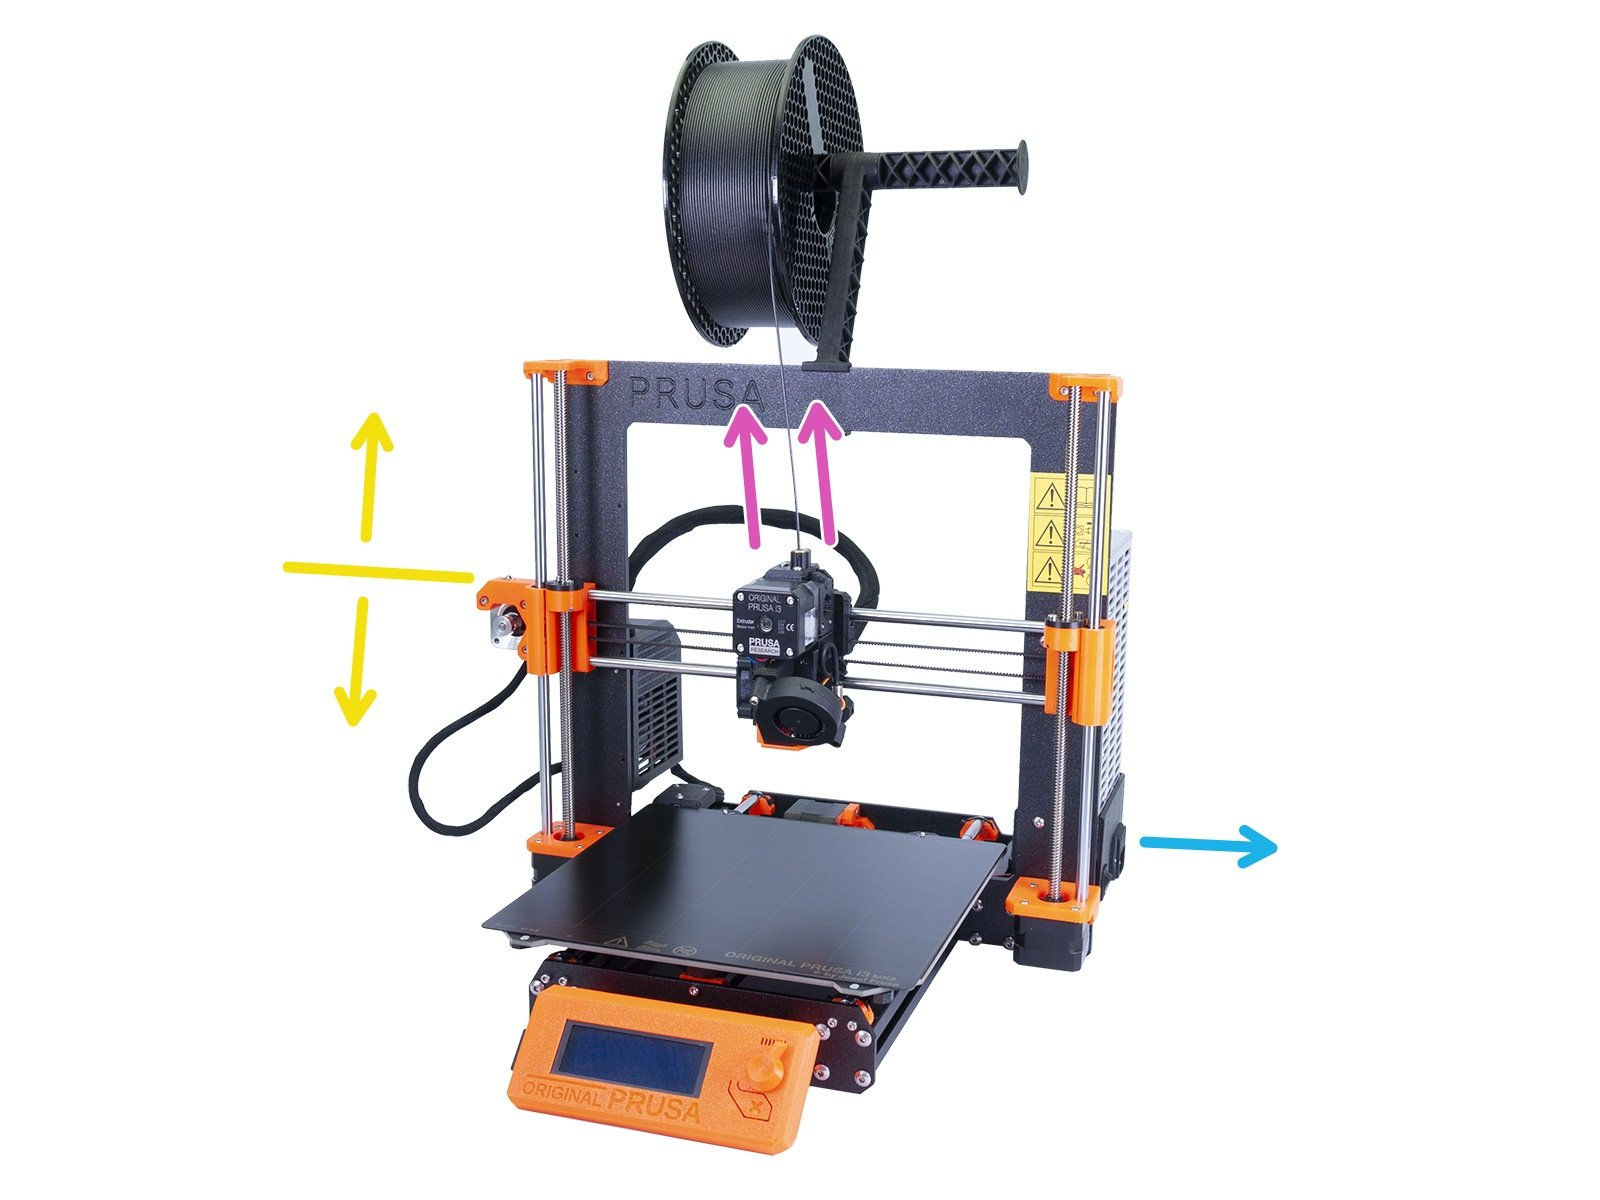
\includegraphics[width=0.5\linewidth]{bilder/Anleitung - X-Achse hoch.jpg}
              \caption[Anleitung: X-Achse auf die Hälfte der Gesamthöhe fahren] { X-Achse auf die Hälfte der Gesamthöhe fahren (Quelle: \autocite{Prusa})}
        \label{X-Achse hoch}
      \end{figure}
    \item Nun folgt das entfernen der Schrauben. Zunächst werden die in \autoref{Schraubi1} dargestellten Schrauben gelöst und entfernt. Im Anschluss werden die grün markierten Schrauben aus \autoref{Schraubi2} entfernt. Abschließend gilt es die orange markierten Schrauben, die den Extruder halten, aus \autoref{Schraubi3} zu entfernen.
      \begin{figure}[h] 
        \centering
        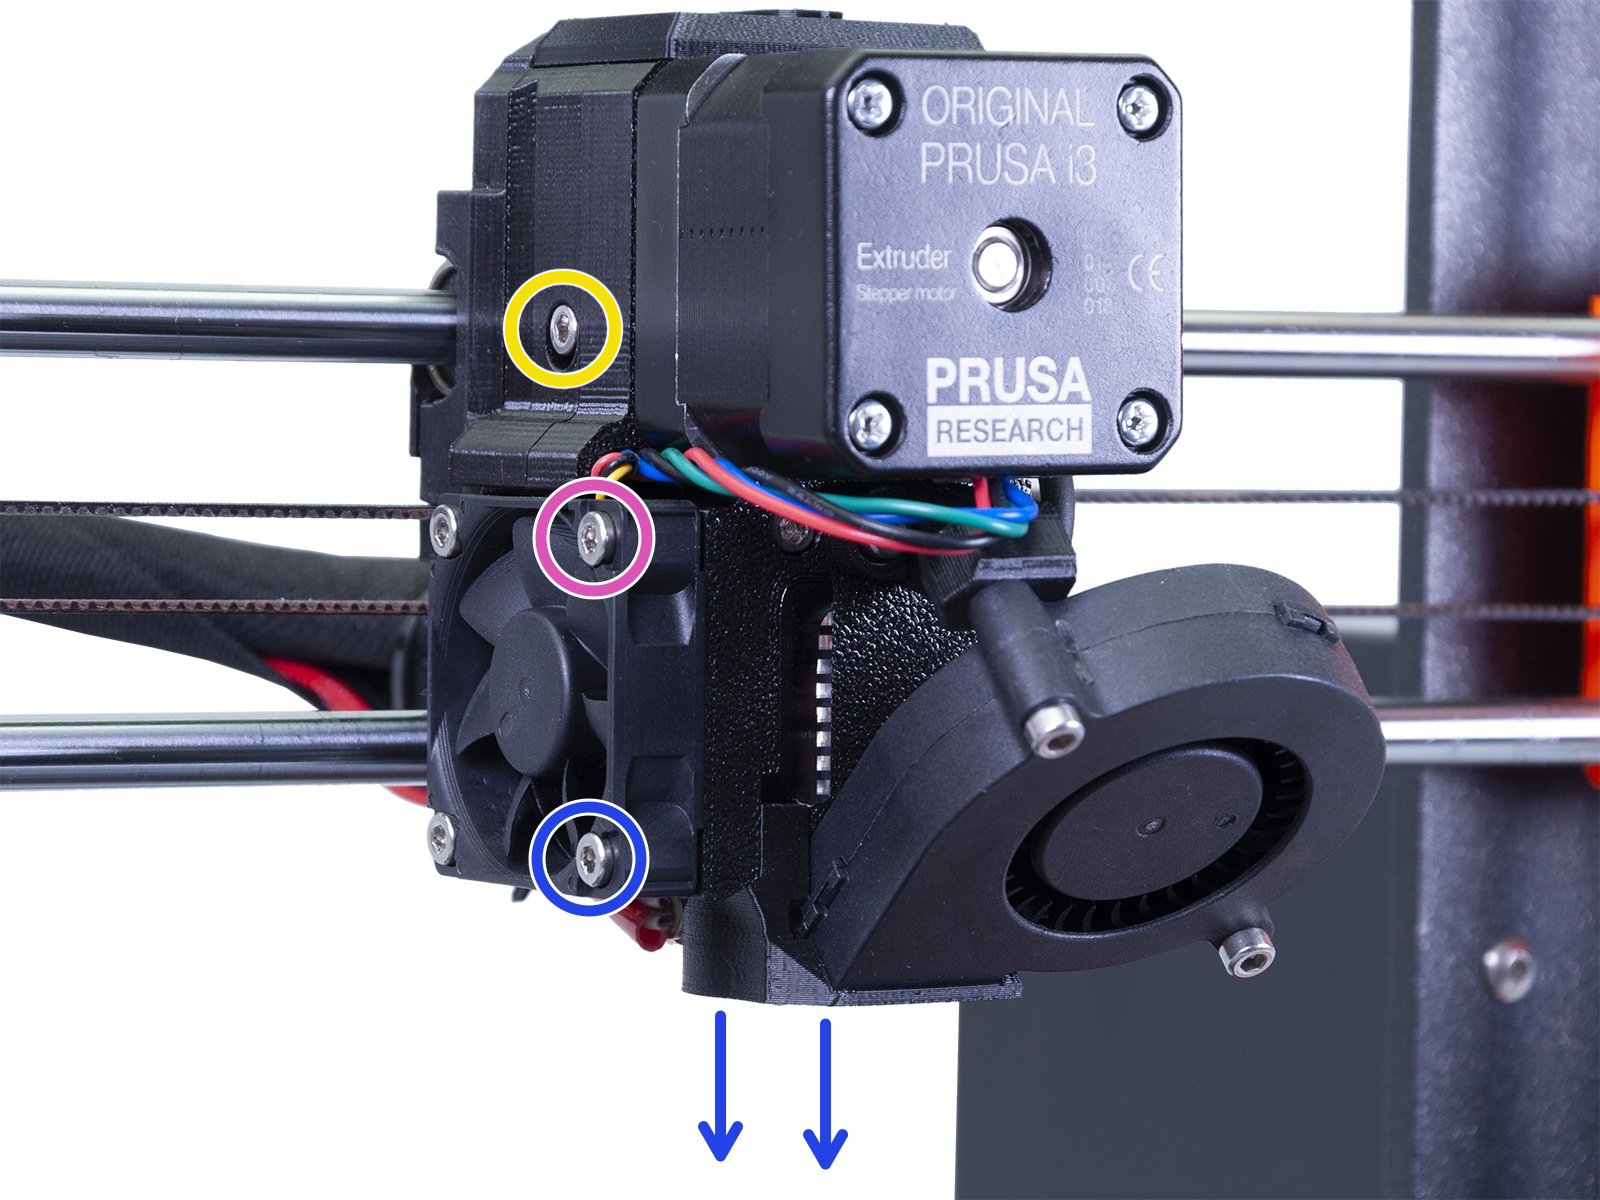
\includegraphics[width=0.5\linewidth]{bilder/Anleitung - Schraubi1.jpg}
              \caption[Anleitung: Gelb, lila und blau markierten Schrauben entfernen] {Gelb, lila und blau markierten Schrauben entfernen (Quelle: \autocite{Prusa})}
        \label{Schraubi1}
      \end{figure}
      \begin{figure}[h]
        \centering
        \begin{subfigure}[b]{0.45\textwidth}
          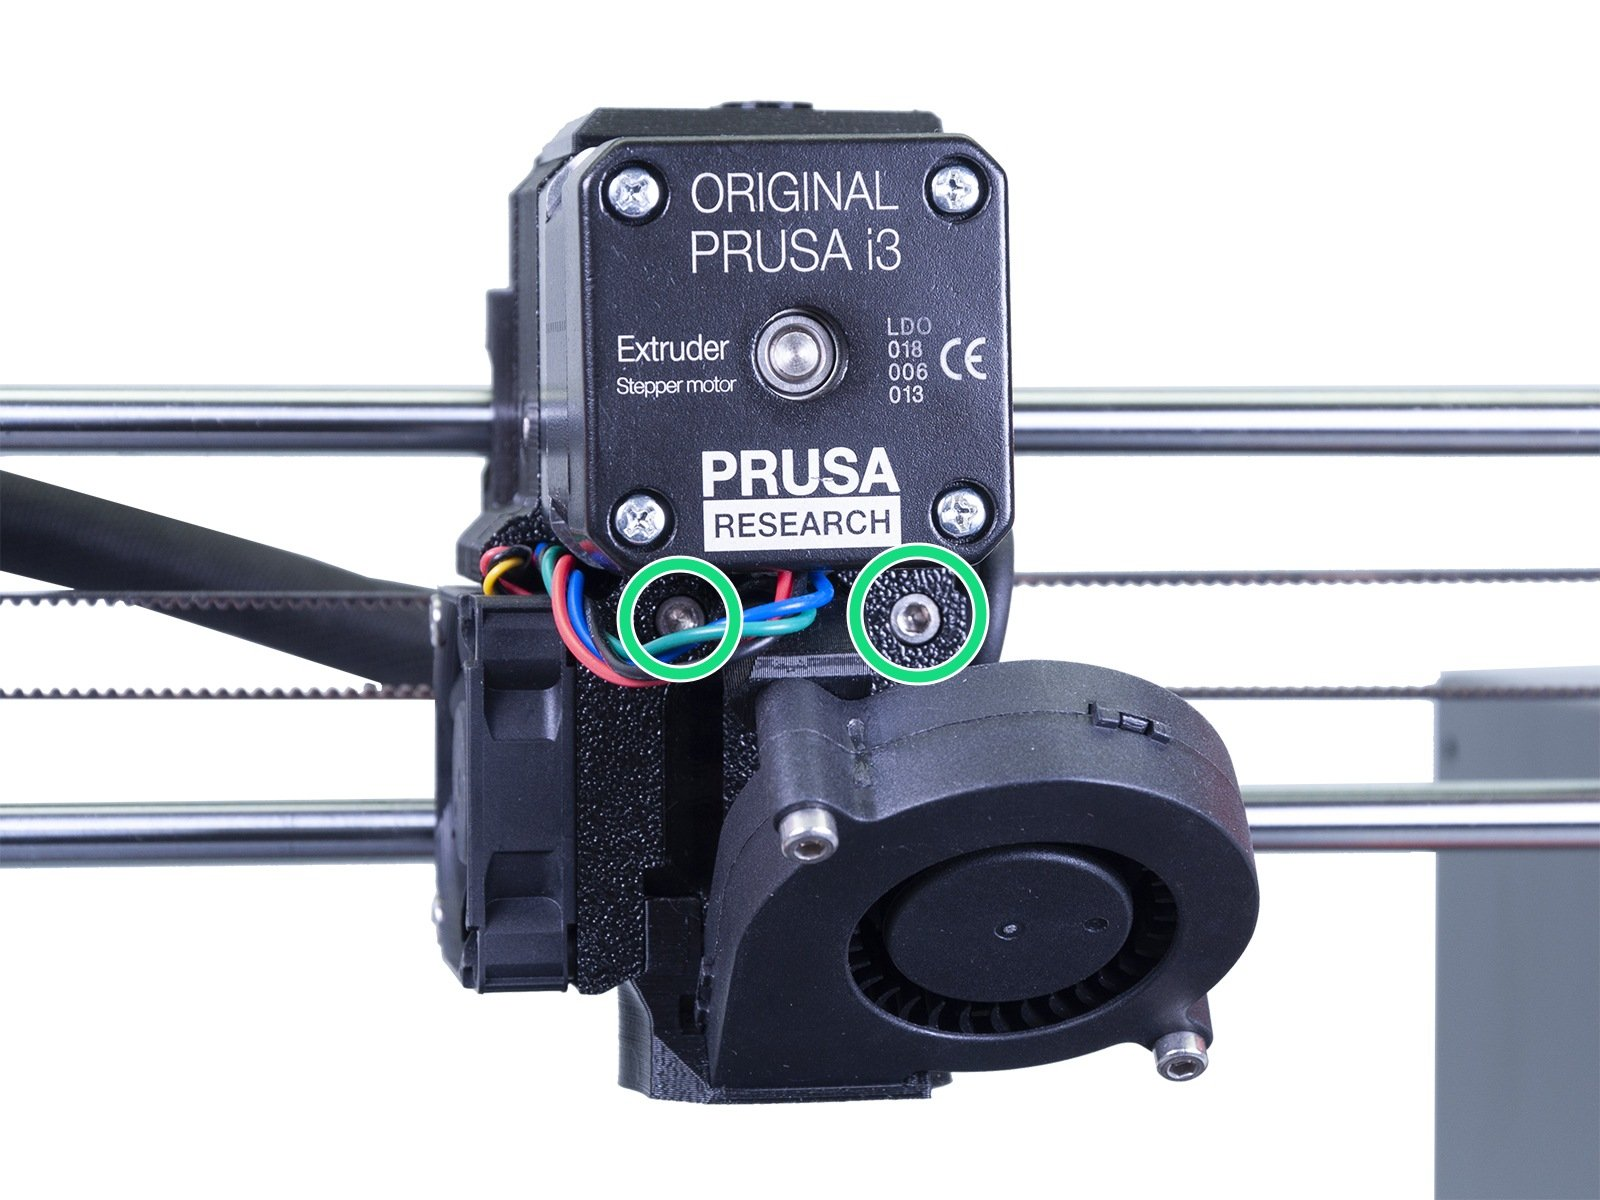
\includegraphics[width=\textwidth]{bilder/Anleitung - Schraubi2.jpg}
          \caption[Anleitung: Grün markierte Schrauben entfernen] {Grün markierte Schrauben entfernen (Quelle: \autocite{Prusa})}
          \label{Schraubi2}
        \end{subfigure}
        \hfill
        \begin{subfigure}[b]{0.45\textwidth}
          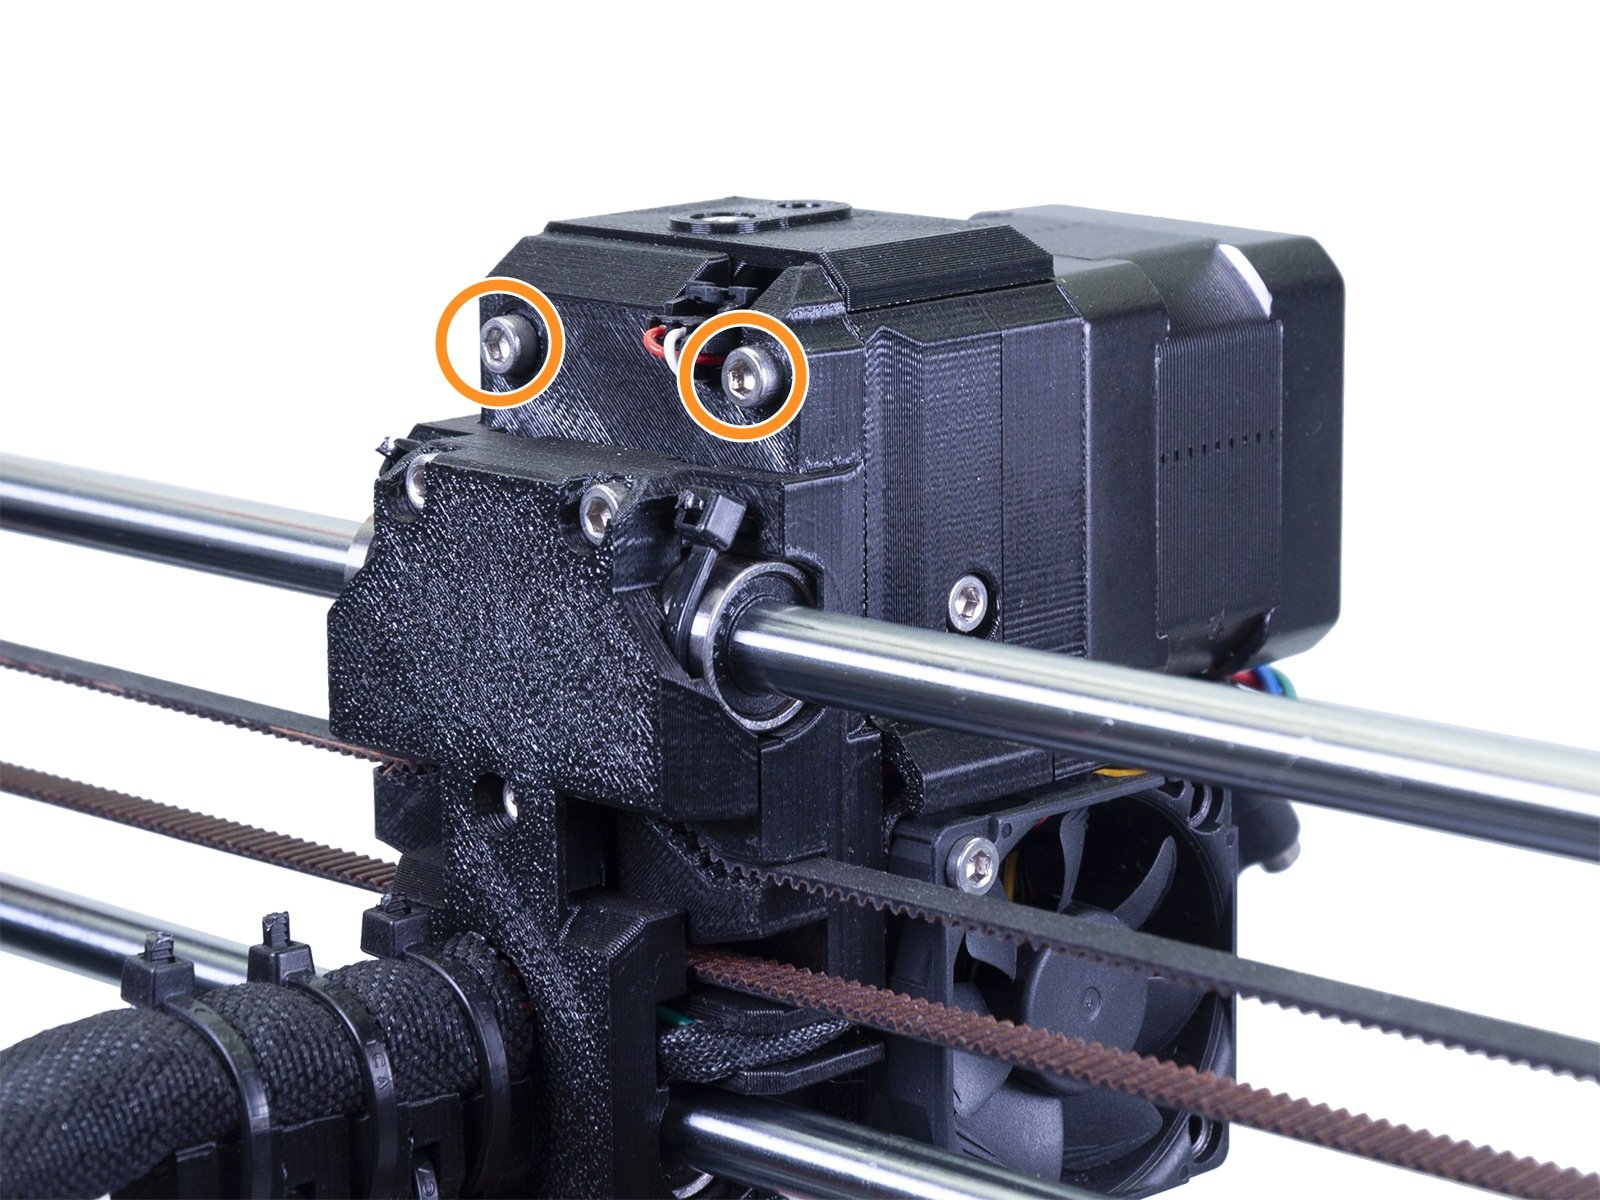
\includegraphics[width=\textwidth]{bilder/Anleitung - Schraubi3.jpg}
          \caption[Anleitung: Orange markierte Schrauben entfernen] {Orange markierte Schrauben entfernen (Quelle: \autocite{Prusa})}
          \label{Schraubi3}
        \end{subfigure}
      \end{figure}
    \item In diesem Schritt wird der Extruder teildemontiert. Dazu Wird vorsichtig der Extrudermotor in Pfeilrichtung (siehe \autoref{Zerlegen1}) gezogen. Sobald dieser lose ist, wird der untere Teil mit herausgezogen. Es muss eine Lücke, wie in \autoref{Zerlegen1} in gelb dargestellt, zu sehen sein.\\
          Nun kann das Hotend vorsichtig von unten entnommen werden (siehe \autoref{Zerlegen2}). Dabei auf die Kabel des Hotends achten, sie dürfen nicht beschädigt werden.
      \begin{figure}[h] 
        \centering
        
      \end{figure}
      \begin{figure}[h]
        \centering
        \begin{subfigure}[b]{0.45\textwidth}
          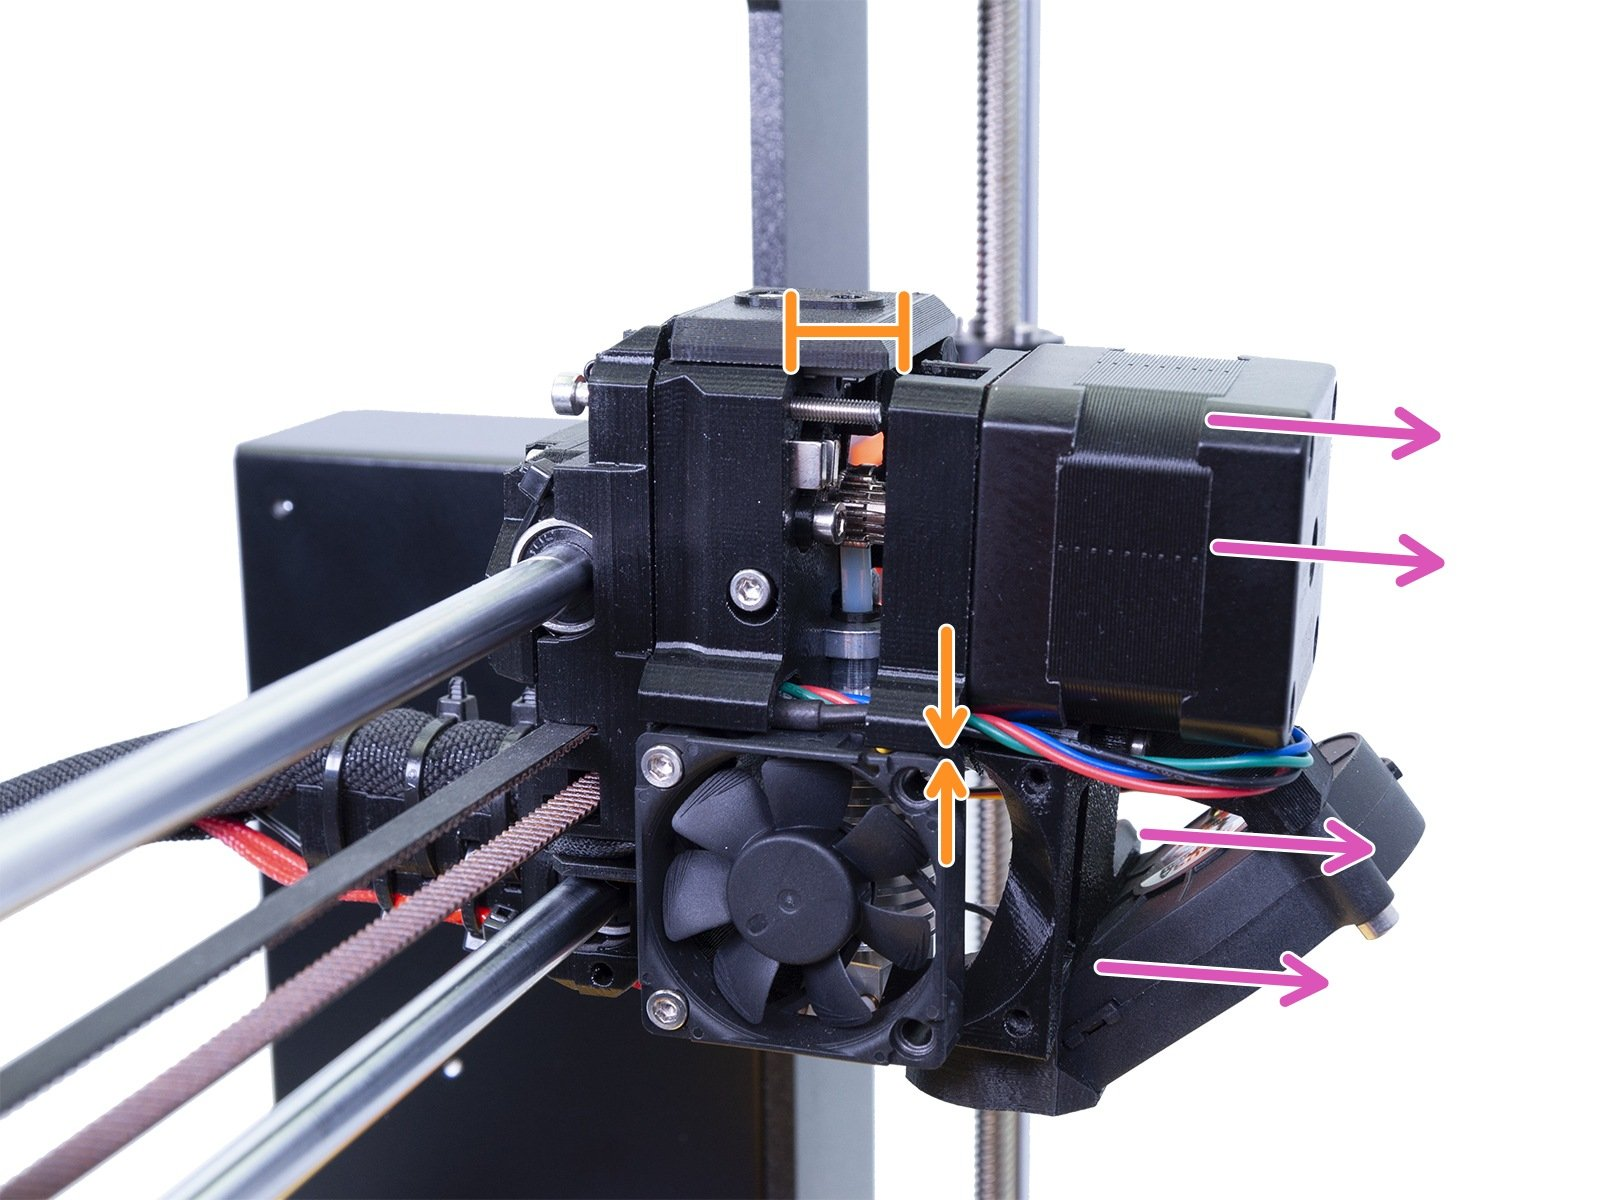
\includegraphics[width=0.5\linewidth]{bilder/Anleitung - Zerlegen1.jpg}
          \caption[Anleitung: Zerlegung des Extruders] {Zerlegung des Extruders (Quelle: \autocite{Prusa})}
        \label{Zerlegen1}
        \end{subfigure}
        \hfill
        \begin{subfigure}[b]{0.45\textwidth}
          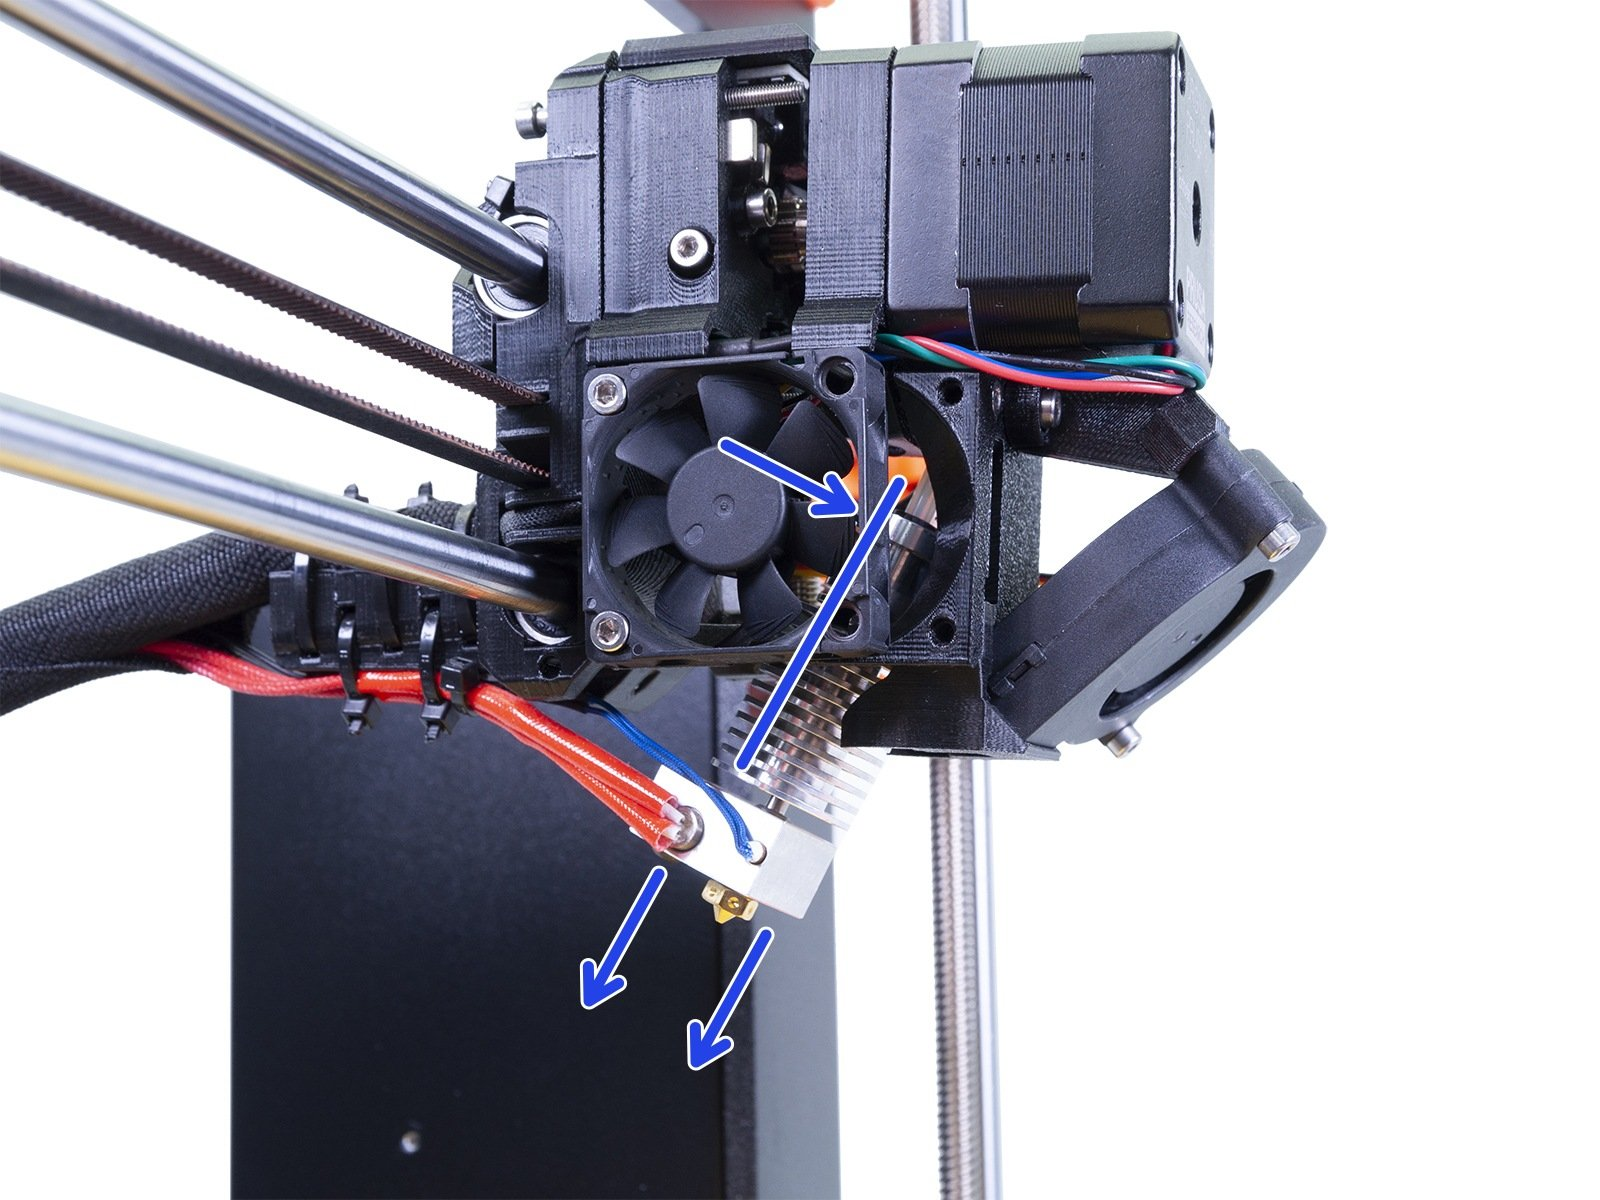
\includegraphics[width=\textwidth]{bilder/Anleitung - Zerlegen2.jpg}
          \caption[Anleitung: Vorsichtige Entnahme des Hotends] {Vorsichtige Entnahme des Hotends (Quelle: \autocite{Prusa})}
          \label{Zerlegen2}
        \end{subfigure}
      \end{figure}
    \item Jetzt kann das PTFE-Schlauchstück mithilfe der entfernt werden. Dazu mit den Fingern den, in \autoref{PTFEEE} mit blauem Pfeil markierten, Ring herunterdrücken und den Schlauch mit der beiliegenden Zange herausziehen. Nun kann die Verstopfung in diesem Schlauchstück mit einem langen, dünnen Hilfsmittel (z.B. einem Imbussschlüssel) entfernt werden.
      \begin{figure}[h] 
        \centering
        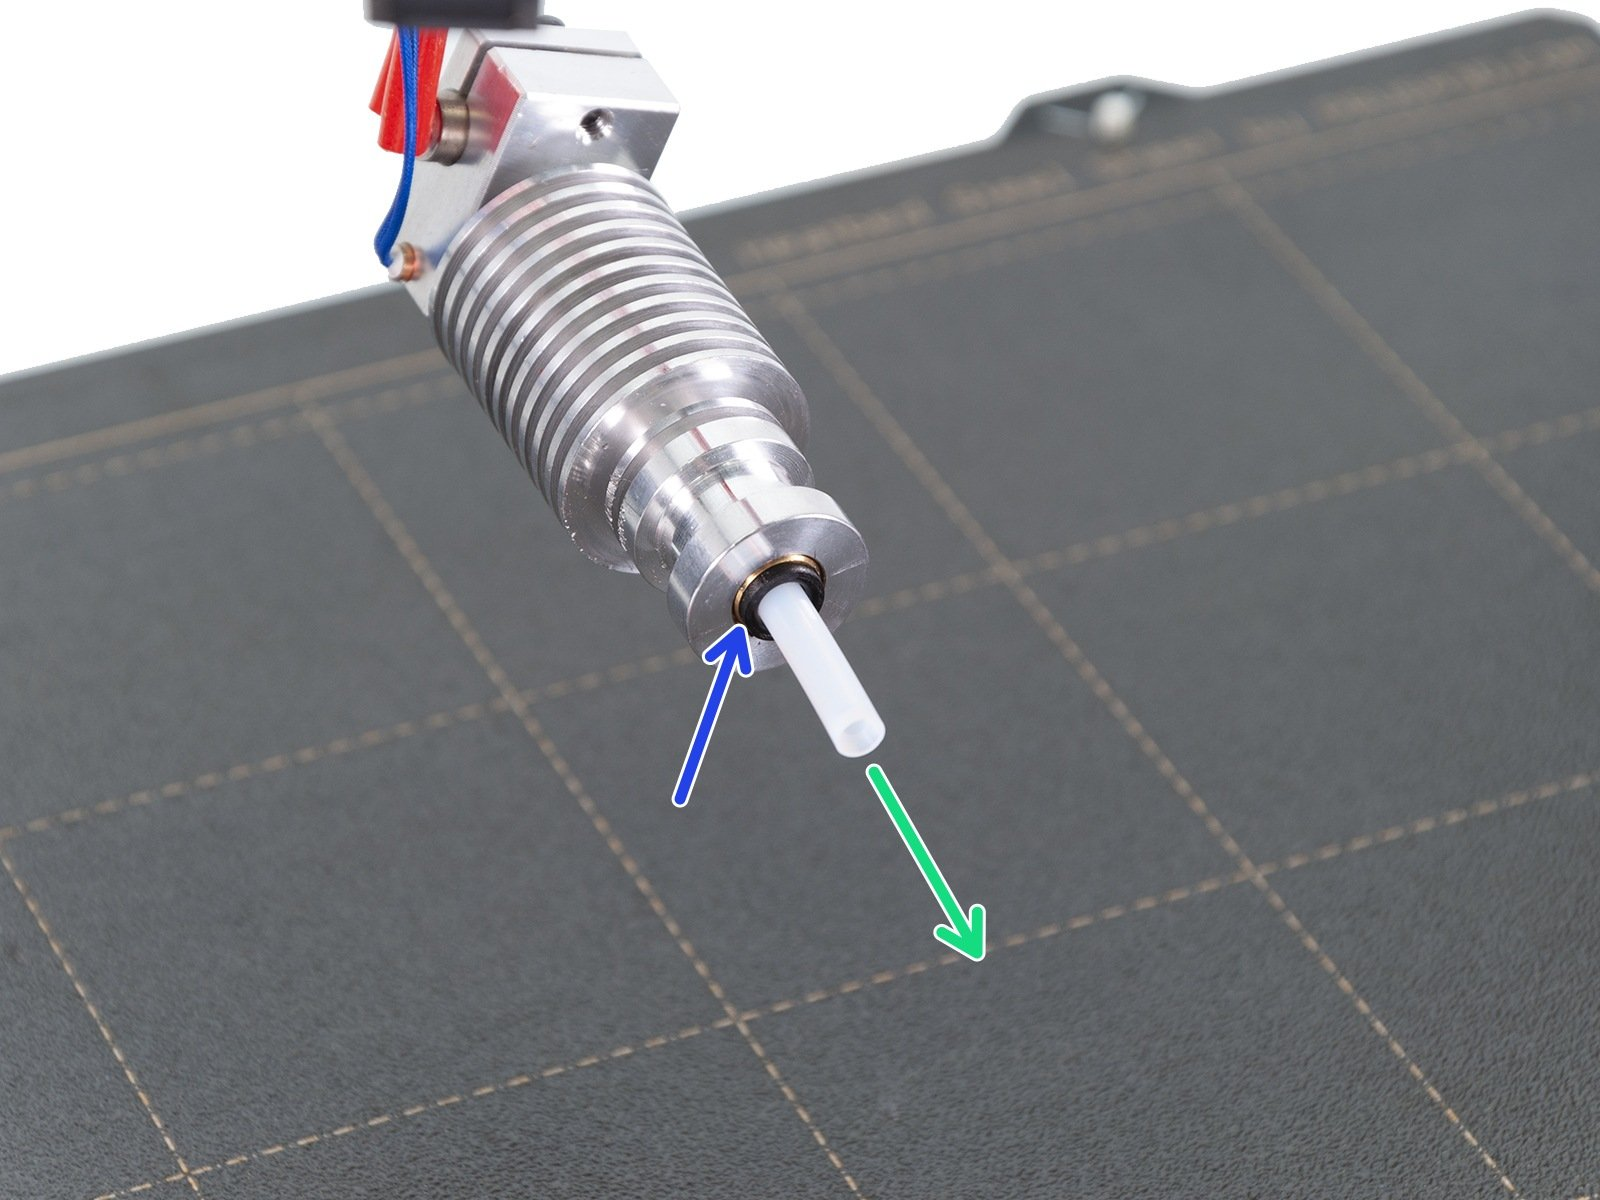
\includegraphics[width=0.5\linewidth]{bilder/Anleitung - Entfernen des PTFE-Schlauchs.jpg}
              \caption[Anleitung: Entfernen des PTFE-Schlauchstücks] {Entfernen des PTFE-Schlauchstücks (Quelle: \autocite{Prusa})}
        \label{PTFEEE}
      \end{figure}
    \item Der Zusammenbau geschieht in umgekehrter Reihenfolge. Wichtig ist, dass der PTFE-Schlauch mit dem angespitztem Ende wieder in den Extruder hineingeführt wird.
    \item Die in gelb dargestellte Schra
    \item Wenn alle Teile wieder zusammengebaut und die Schrauben wieder festgezogen sind, kann die Düse auf 180°C aufgeheizt werden. Sobald die Temperatur erreicht ist, wird das Ende der Filamentrolle schräg mit der Zange abgeschnitten. Um das  
\end{itemize}

\end{document}
